\chapter{Geometría Diferencial de las Curvas y Superficies}

\section{Movimientos Rígidos}

Cuando estudiamos Geometría, buscamos entender las propiedades de ciertos objetos (geométricos) que permanecen invariantes bajo ciertos movimientos. En esta primera parte, nos interesará estudiar propiedades de las curvas bajo la acción de movimientos rígidos

\begin{defn}
Un \textbf{movimiento euclídeo} (también llamado rígido) es una función $f:\RR^n\to\RR^n$ que preserva las distancias. Es decir $||f(x)-f(y)||=||x-y||$ para todos $x,y\in\RR^n$. Al conjunto de movimientos euclídeos de $\RR^n$ lo denotaremos por $\Iso(n)$.
\end{defn}

\begin{obs}
Notar que, por definición, la distancia entre dos puntos es un invariante euclídeo.
\end{obs}

Nuestro primer objetivo será caracterizar a los movimientos rígidos. Para eso, recordemos un par de hechos básicos de Álgebra Lineal. Una matriz $A\in\GL_n(\RR)$ se dice \textbf{ortogonal} si satisface que $AA^t=I$. Se define el \textbf{grupo ortogonal} como $$O(n)=\{A\in\GL_{n}(\RR) : AA^{t}=I\}$$ Es fácil probar que $O(n)$ es de hecho un grupo. Recordemos también que $A\in\GL_n(\RR)$ es ortogonal si y sólo si $\langle Ax,Ay\rangle = \langle x,y\rangle$ para todos $x,y\in\RR^n$. Por lo tanto, si $x\in\RR^n$ y $A\in O(n)$ tenemos que $\norm{Ax}^2 = \langle Ax,Ax\rangle = \langle x,x\rangle = \norm{x}^2$. Por lo tanto, $\norm{Ax}=\norm{x}$.

Notemos que si $A\in O(n)$ y $b\in\RR^n$, entonces la función $f:\RR^n\to\RR^n$ dada por $f(x)=Ax+b$ es un movimiento eucídeo. En efecto, esto se debe a que si $x,y\in\RR^n$, entonces $\norm{f(x)-f(y)} = \norm{A(x-y)} = \norm{x-y}$.

\begin{lem}
\label{lem::ptomedio}
Sean $x,y,z\in\RR^n$. Si $\norm{x-z} = \norm{z-y} = \frac{1}{2}\norm{x-y}$, entonces $z=\dfrac{x+y}{2}$. Esto es, la existencia y unicidad del punto medio entre dos puntos $x,y\in\RR^n$.
\begin{proof}
Si $x=z$ o $y=z$, no hay nada que probar. Por otra parte, si $z\neq x,y$, tenemos que $\norm{x-z}+\norm{z-y} = \norm{x-y} = \norm{(x-z)+(z-y)}$. Es decir, se da la igualdad en la desigualdad triangular. Pero esto implica que existe un escalar $\lambda\in\RR_{>0}$ tal que $x-z = \lambda(z-y)$. Tomando norma, se sigue que $|\lambda|=1$ y así $x-z=z-y$. Por lo tanto, $z=\dfrac{x+y}{2}$. Como queríamos probar.
\end{proof}
\end{lem}

\begin{teo}[Mazur-Ulam]
Sea $f:\RR^n\to\RR^n$. Entonces, $f$ es un movimiento euclídeo si y sólo si es de la forma $f(x)=Ax+b$ con $A\in O(n)$, $b\in\RR^n$. Más aún, esta expresión es única. Es decir, si $f(x)=A'x+b'$ con $A'\in O(n)$ y $b'\in\RR^n$, entonces $A=A'$ y $b=b'$.
\begin{proof}
\hfill

$(\Longleftarrow)$ Ya lo probamos.

$(\Longrightarrow)$ Probemos primero que $f$ satisface la siguiente identidad: \begin{equation}f((1-t)x+ty) = (1-t)f(x) + tf(y) \;\forall t\in\RR, x,y\in\RR^n\label{eq::afin}\end{equation}

Veamos que para $t=\dfrac{1}{2}$ se satisface ~\ref{eq::afin}. En efecto, como $f$ es euclídea, se cumple que: $$\norm{f(x)-f\left(\dfrac{x+y}{2}\right)} = \dfrac{1}{2}\norm{f(x)-f(y)} = \norm{f\left(\dfrac{x+y}{2}\right)-f(y)}$$ y por el Lema anterior~\ref{lem::ptomedio} se sigue que $f\left(\dfrac{x+y}{2}\right)$ es el punto medio entre $f(x)$ y $f(y)$.

Veamos ahora que la identidad ~\ref{eq::afin} se satisface para los racionales diádicos. Es decir, $t=\dfrac{\ell}{2^n}$ donde $\ell\in\{0,1,\ldots, 2^n\}$ y $n\in\NN_{0}$. Para esto, procederemos por inducción en $n$. Si $n=0$ es trivial. Supongamos entonces $n>0$ y $\ell\in\{0,1,\ldots, 2^n\}$. Si $\ell$ es par, entonces $t=\dfrac{(\ell/2)}{2^{n-1}}$ y por hipótesis inductiva ya estamos. Si no, podemos escribir $\ell = 2\ell'+1$. En ese caso, tenemos que $\dfrac{\ell'}{2^{n-1}} < \dfrac{\ell}{2^n} < \dfrac{\ell'+1}{2^{n-1}}$ y $\dfrac{\ell}{2^n}$ es el promedio de los extremos. Por hipótesis inductiva, sabemos que se cumplen: \begin{align*}f\left(\left(1-\dfrac{\ell'}{2^{n-1}}\right) x + \dfrac{\ell'}{2^{n-1}}y\right) &= \left(1-\dfrac{\ell'}{2^n}\right) f(x) + \dfrac{\ell'}{2^{n-1}}f(y) \\ f\left(\left(1-\dfrac{\ell'+1}{2^{n-1}}\right) x + \dfrac{\ell'+1}{2^{n-1}}y\right) &= \left(1-\dfrac{\ell'+1}{2^n}\right) f(x) + \dfrac{\ell'+1}{2^{n-1}}f(y) \end{align*} Sumando ambas ecuaciones y usando que para $t=\dfrac{1}{2}$ el resultado vale, se sigue lo deseado.

Ahora bien, $f$ es continua por ser una isometría. Por la continuidad y la densidad de los diádicos en el intervalo $[0,1]$ se sigue que se satisface la identidad ~\ref{eq::afin} para todo $t\in [0,1]$. Si $t>1$ se sigue que $y$ está entre $x$ y $z=(1-t)x+ty$ con $y = \left(1-\dfrac{1}{t}\right)x + \dfrac{1}{t}z$ y ahí vale el resultado pues $\dfrac{1}{t}\in[0,1]$. Para $t<0$ es análogo.

Consideremos entonces la función $g:\RR^n\to\RR^n$ dada por $g(x)=f(x)-f(0)$. Veamos que $g$ es una transformación lineal. Notemos que por la identidad ~\ref{eq::afin} se tiene que $f(tx)=f((1-t)0 + tx) = (1-t)f(0) + tf(x)$. Manipulando esa ecuación obtenemos $g(tx)=f(tx)-f(0)=t(f(x)-f(0))=tg(x)$. Ahora bien, notemos que $\dfrac{g(x+y)}{2}=g\left(\dfrac{x+y}{2}\right) = f\left(\dfrac{x+y}{2}\right)-f(0) = \dfrac{f(x)}{2}+\dfrac{f(y)}{2}-f(0) = \dfrac{g(x)+g(y)}{2}$. Como $g$ es lineal, debe existir una matriz $A\in\RR^{n\times n}$ tal que $g(x)=Ax$ y así tenemos que $f(x)=Ax+f(0)$.
Por lo tanto, sabemos que $\norm{A(x-y)} = \norm{f(x)-f(y)} = \norm{x-y}$. En particular $A$ es inversible. Además, $\norm{A(x-y)}^2 = \norm{Ax}^2 + \norm{Ay}^2 - 2\langle Ax,Ax\rangle$ y $\norm{x-y}^2 = \norm{x}^2 + \norm{y}^2 - 2\langle x,y\rangle$. Se sigue entonces que $\langle Ax,Ay\rangle = \langle x,y\rangle$. Esto implica que $A$ es ortogonal, como queríamos.

Para concluir, si $f(x)=Ax+b=A'x+b'$, entonces $b=f(0)=b'$ y así $(A-A')x=0$ para todo $x\in\RR^n$, lo que implica que $A=A'$.
\end{proof}
\end{teo}

\begin{cor}
El conjunto $\Iso(n)$ es un subgrupo del grupo de las biyecciones $\RR^n\to\RR^n$.
\begin{proof}
Claramente la identidad es una isometría. Si $f,g\in\Iso(n)$, entonces por el Teorema de Mazur-Ulam, $f(x)=A_fx+b_f$, $g(x)=A_gx+b_g$ y entonces la composición $(f\circ g)(x) = A_f(A_gx+b_g)+b_f = A_fA_gx + (A_fb_g+b_f)$ también es una isometría pues $A_fA_g\in O(n)$ por ser $O(n)$ un grupo. Por último, como la inversa de $A_f$ es $A_f^t$ es fácil verificar que si $g(x) = A_f^t x - A_f^t b_f$ tenemos que $f\circ g = g\circ f = 1$, y así $g\in\Iso(n)$ es la inversa de $f$.
\end{proof}
\end{cor}

Por el Teorema de Mazur-Ulam, podemos escribir a cada $f\in\Iso(n)$ de la forma $f(x)=A_fx+b_f$ con $A_f\in O(n)$ y $b_f\in\RR^n$. Como $A_f\in O(n)$ tenemos que $A_f A_f^t = I$ y así debemos tener que $\det A_f = \pm 1$. Consideramos $\Iso^+(n) = \{f\in\Iso(n) : \det A_f = 1\}$ y $\Iso^-(n) = \{f\in\Iso(n):\det A_f = -1\}$. Notemos que claramente $\Iso^+(n)\subseteq\Iso(n)$ es un subgrupo. Además, si recordamos que el \textbf{grupo especial ortogonal} se define como $\mathrm{SO}(n)=\{A\in O(n) : \det A = 1\}$ se tiene que $\Iso^+(n)$ se corresponde con $\mathrm{SO}(n)$. A las transformaciones de $\Iso^+(n)$ se las denomina \textbf{movimientos directos}. Es claro que $\Iso^+(n)\sqcup\Iso^-(n)=\Iso(n)$ y que $\Iso^+(n)$ está en biyección con $\Iso^-(n)$ simplemente tomando $M\in O(n)$ con $\det M = -1$ y considerando la aplicación $Ax+b\mapsto MBx+b$. Finalmente, es fácil ver que la aplicación $\pi:\Iso(n)\to O(n)$ dada por $\pi(f)=A_f$ es un morfismo de grupos cuyo núcleo consiste en las traslaciones.

\section{Curvas en Espacios Euclídeos}

Para afrontar el aspecto diferencial del estudio de las curvas necesitaremos asumir alguna condición de regularidad con respecto a las derivadas. De ahora en más, fijemos $k\in \NN_0\cup\{\infty\}$ a gusto y cada vez que digamos \textit{diferenciable} nos estaremos refiriendo a \textit{de clase} $\mathscr{C}^k$. Además, cada vez que escribamos $(a,b)$ nos referiremos a un intervalo abierto donde posiblemente los extremos son $\pm\infty$.

\begin{defn}
Una \textbf{curva paramétrica} en $\RR^n$ es un conjunto $\mathscr{C}\subseteq\RR^n$ junto con una función diferenciable $\sigma:I\to\RR^n$ (donde $I\subseteq\RR$ es un intervalo abierto) de modo tal que la imagen de $\sigma$ es $\mathscr{C}$. Se dice que $\sigma$ es una \textbf{parametrización} de la curva. La \textbf{traza} de una curva es la imagen de una parametrización de la misma. Decimos que la parametrización es \textbf{regular} en $t\in I$ si $\sigma'(t)\neq 0$. En caso contrario, se dice que la curva es \textbf{singular} en $t$. Si la curva es regular en todo punto de $I$ decimos que es una \textbf{curva regular}.
\end{defn}

\begin{ex}\hfill

\begin{itemize}\item Si $p\in\RR^n, v\in\RR^n\smallsetminus\{0\}$, la curva parametrizada por $\alpha:I\to\RR^n$, $\alpha(t)=p+tv$ es un segmento de recta que pasa por $p$ y tiene dirección $v$. Es regular pues $\alpha'(t) = v$. Esta curva es de clase $\mathscr{C}^\infty$.
\item Los gráficos de funciones son otro ejemplo clásico de curvas parametrizadas. Si $f:I\to\RR$ es una función de clase $\mathscr{C}^k$ entonces el gráfico $$\mathrm{Graf}(f) = \{(t,f(t)) : t\in I\}$$ es una curva parametrizada por $\alpha:I\to\RR^2$, $\alpha(t)=(t,f(t))$. Trivialmente es regular pues $\alpha'(t)=(1,f'(t))\neq (0,0)$ y es de clase $\mathscr{C}^k$.
\item Podemos dar curvas planas en términos de \textbf{coordenadas polares}. Es decir, parametrizamos $\alpha:I\to\RR^n$, $\alpha(\theta)=(\rho(\theta)\cos(\theta),\rho(\theta)\sen(\theta))$, donde $\rho:I\to\RR_{>0}$ es una función de clase $\mathscr{C}^k$. Veamos que $\alpha$ parametriza a una curva regular. En efecto, $\alpha'(\theta) = \rho'(\theta)(\cos(\theta),\sen(\theta)) + \rho(\theta)(-\sen(\theta),\cos(\theta))$. Como $(\cos(\theta),\sen(\theta))$ y $(-\sen(\theta),\cos(\theta))$ son vectores unitarios ortogonales, por Pitágoras tenemos que $\norm{\alpha'(\theta)}^2 = \abs{\rho(\theta)}^2 + \abs{\rho'(\theta)}^2$. Eso implica que $\alpha'$ sólo se anula si $\rho(\theta)=\rho'(\theta)=0$ y eso no puede pasar pues $\rho$ siempre es positiva.
\item La parametrización es muy importante. El conjunto $\mathscr{C}=\{(x,y)\in\RR^2:x=y\}$ admite muchas parametrizaciones. Por ejemplo, $\alpha,\beta:\RR\to\RR^2$, $\alpha(t)=(t,t)$ y $\beta(t)=(t^3,t^3)$. La primera es regular pues $\alpha'(t)=(1,1)$ mientras que la segunda no, pues $\beta'(t)=(3t^2,3t^2)$ es singular en $t=0$.
\item Consideremos la curva parametrizada por $\alpha:\RR\to\RR^2$, $\alpha(t)=(t^2,t^3)$. Esta curva no es regular, pues $\alpha'(t)=(2t,3t^2)$ es singular en $t=0$. Gráficamente, se puede ver que en el punto $t=0$ la curva no admite una recta tangente.

\textcolor{red}{Agregar dibujos de cada ejemplo}
\end{itemize}
\end{ex}

\begin{lem}
Sea $\sigma:(a,b)\to\RR^n$ una curva regular. Si $c\in (a,b)$, entonces existe $\eps>0$ tal que $(c-\eps,c+\eps)\subseteq (a,b)$ y $\left.\sigma\right|_{(c-\eps,c+\eps)}$ es inyectiva. Es decir, toda curva es localmente inyectiva.
\begin{proof}
Supongamos que el enunciado es falso. Es decir, existe $c\in (a,b)$ tal que para todo $m\in\NN$, en cada intervalo $\left(c-\dfrac{1}{m},c+\dfrac{1}{m}\right)$ existen $x_m<y_m$ de tal modo que $\sigma(x_m)=\sigma(y_m)$ y además $\displaystyle\lim_{m\to\infty}x_m = c = \displaystyle\lim_{m\to \infty}y_m$. Tomemos $i\in\{1,\ldots , n\}$. Como $\sigma_i(x_m)=\sigma_i(y_m)$, por el Teorema del Valor Medio, existe $\xi_m^{(i)}\in (x_m,y_m)$ tal que $\sigma_i'(\xi_m^{(i)})=0$. Claramente, $\lim_{m\to\infty}\xi_m^{(i)}=c$. Por lo tanto (asumiendo una regularidad de clase $\mathscr{C}^1$ al menos) tendremos que $0=\displaystyle\lim_{m\to\infty}\sigma_i'(\xi_m^{(i)})=\sigma_i'(c)$. Por lo tanto, $\sigma'(c)=0$, contradiciendo que $\sigma$ es una curva regular.
\end{proof}
\end{lem}

\begin{cor}
Si $\sigma:(a,b)\to\RR^n$ es una curva regular, entonces todo punto de $\RR^n$ tiene un número finito de preimágenes en cada intervalo cerrado y acotado $[c,d]\subseteq (a,b)$.
\begin{proof}
En virtud del lema anterior, para cada $x\in [c,d]$ existe $\eps_x>0$ tal que $\left.\sigma\right|_{(x-\eps_x,x+\eps_x)}$ es inyectiva. El conjunto $\{(x-\eps_x,x+\eps_x) : x\in [c,d]\}$ es claramente un cubrimiento por abiertos de $[c,d]$, y por la compacidad, deben existir $x_1,\ldots , x_\ell$ de modo tal que $[c,d]\subseteq\displaystyle\bigcup_{i=1}^{\ell} (x_i-\eps_{x_i},x_i+\eps_{x_i})$. Por lo tanto, si $v\in\RR^n$, se sigue que $$\sigma^{-1}(v)\cap [c,d] \subseteq \displaystyle\bigcup_{i=1}^\ell (x_i-\eps_{x_i},x_i+\eps_{x_i})\cap \sigma^{-1}(v)$$ Como la restricción de $\sigma$ a cada intervalo $(x_i-\eps_{x_i},x_i+\eps_{x_i})$ es inyectiva, esa unión tiene a lo sumo $\ell$ elementos. Y estamos.
\end{proof}
\end{cor}

\begin{ex}
Por lo general es falso que la fibra sea finita si no nos restringimos a un compacto. Por ejemplo, $\sigma:\RR\to\RR^2$ dada por $\sigma(t)=(\cos t,\sen t)$ tiene fibra $\sigma^{-1}((x_0,y_0)) = \{t_0 + 2k\pi : (\cos(t_0),\sen(t_0))=(x_0,y_0), k\in\ZZ\}$, que es infinita para cualquier punto $(x_0,y_0)$ en la circunferencia unitaria. Esto nos muestra que una curva posee más información que solamente su traza. Además, tenemos varias parametrizaciones distintas que describen una misma traza, como por ejemplo $\sigma_1:(0,2\pi)\to \RR^2$ dada por $\sigma_1(t)=(\cos(t),\sen(t))$ o $\sigma_2:(0,1)\to \RR^2$ dada por $\sigma_2(t)=(\cos(2\pi t),\sen(2\pi t))$.
\begin{figure}[h]
	\centering
		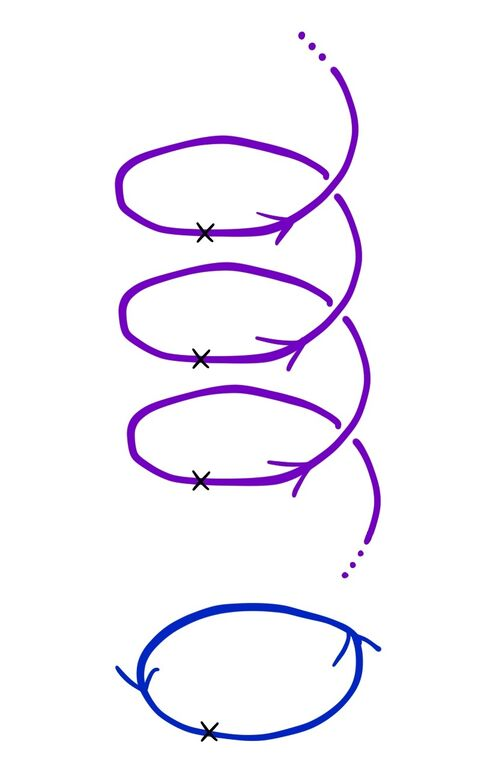
\includegraphics[width=0.25\textwidth]{C:/Users/Nacho/Documents/Latex/Facultad/GeometriaProyectiva/GeoProyectiva/revestimientos1.jpg}
	\caption{Una parametrización de $S^1$ cuya fibra no es finita}
	\label{fig:revestimientos1}
\end{figure}
\end{ex}

\begin{defn}
Una \textbf{reparametrización} es una función $u:(a,b)\to (c,d)$ biyectiva, diferenciable y con inversa diferenciable.
\end{defn}

\begin{defn}
Si $\sigma:(a,b)\to\RR^n$ es una curva regular y $u:(c,d)\to (a,b)$ es una reparametrización, entonces $\sigma\circ u:(c,d)\to\RR^n$ es una curva regular y se dice que $\sigma\circ u$ es una \textbf{reparametrización} de $\sigma$. Decimos $u$ que es una \textbf{reparametrización directa} si $u'(t)>0 \;\forall t\in (c,d)$.
\end{defn}

Como ya vimos, una curva posee más información que meramente su traza. Vamos a estudiar propiedades de las curvas que sean invariantes por movimientos rígidos y por reparametrización.

\section{Invariantes}

\begin{defn}
Sea $\mathscr{C}(n)$ el conjunto de pares $(\sigma,s_0)$ con $\sigma_I\to\RR^n$ una curva regular y $s_0\in I$. Un miembro del conjunto $\mathscr{C}(n)$ se llama un \textbf{elemento de curva}.
\end{defn}

\begin{defn}
Un \textbf{invariante escalar} es una función $V:\mathscr{C}(n)\to\RR$ que permanece invariante bajo movimientos rígidos y reparametrizaciones directas. Es decir, tal que $V(f\circ\sigma,s_0) = V(\sigma,s_0)$ para todo $f\in\Iso^+(n)$ y además $V(\sigma\circ u,u^{-1}(s_0)) = V(\sigma,s_0)$ para toda reparametrización directa $u:(a,b)\to \mathrm{Dom}\sigma$.
\end{defn}

\begin{defn}
Un \textbf{invariante vectorial} es una función $V:\mathscr{C}(n)\to\RR^n$ que cumple que $V(f\circ\sigma,s_0)=A_f V(\sigma,s_0)$ para todo $f\in\Iso^+(n)$ y $V(\sigma\circ u,u^{-1}(s_0)) = V(\sigma,s_0)$ para toda reparametrización directa $u:(a,b)\to\mathrm{Dom}\sigma$.
\end{defn}

\begin{comm}
Dado un grupo $G$ y dos conjuntos $X,Y$ provistos de acciones $G\acts X$, $G\acts Y$, una función $f:X\to Y$ se dice \textbf{equivariante} si $f(g\cdot x)=g\cdot f(x)$ para todos $x\in X,g\in G$. Es decir, el siguiente diagrama conmuta:

\begin{center}
\begin{tikzcd}
X \arrow[]{r}[font=\normalsize]{\cdot g}\arrow[]{d}[font=\normalsize, left]{f} & X\arrow[]{d}[font=\normalsize, right]{f} \\
Y \arrow[]{r}[font=\normalsize]{\cdot g} & Y
\end{tikzcd}
\end{center}

Si consideramos a $\Iso^+(n)$ actuando en $\mathscr{C}(n)$ vía $f\cdot (\sigma,s_0) = (f\circ\sigma,s_0)$ y a $\Iso^+(n)$ actuando en $\RR^n$ por $f\cdot x = A_f x$, entonces un invariante vectorial $V:\mathscr{C}(n)\to\RR^n$ es simplemente un morfismo equivariante respecto de estas acciones que es invariante bajo reparametrizaciones directas.
\end{comm}

\begin{defn}
Dos elementos de curva $(\sigma,s_0),(\tau,t_0)$ definen el mismo \textbf{germen} si existe $I\subseteq \mathrm{Dom}\sigma\cap\mathrm{Dom}\tau$ tal que $s_0=t_0\in I$ y además $\left.\sigma\right|_{I} = \left.\tau\right|_{I}$. Lo notaremos $(\sigma,s_0)\sim (\tau,t_0)$. Claramente $\sim$ es una relación de equivalencia y llamaremos al conjunto de clases de equivalencia (es decir, $\mathscr{C}(n)/\sim$) el conjunto de \textbf{gérmenes}. Si $x\in\RR^n$, denotamos por $\mathcal{O}_x$ al conjunto de gérmenes en $x$, es decir, las clases de equivalencia $[(\sigma,s_0)]$ tales que $\sigma(s_0)=x$ (notar que esto no depende del representante $(\sigma,s_0)$). Los gérmenes nos proveerán del contexto adecuado para estudiar propiedades locales. \textcolor{red}{Agregar dibujo de dos curvas en un mismo germen}
\end{defn}

\begin{obs}\label{obs::germenderivadas}
Sean $(\sigma,s_0)$ y $(\tau,t_0)$ dos elementos de un mismo germen. Entonces, $\sigma'(s_0)=\tau'(t_0)$. En efecto, notemos que como están en el mismo germen existe un intervalo $I$ tal que $s_0=t_0$ y $\left.\sigma\right|_{I}=\left.\tau\right|_{I}$, y así el cociente incremental coincide en un entorno de $s_0=t_0$. Tomando límite se sigue lo deseado.
\end{obs}

\begin{defn}
Un invariante $V$ (escalar o vectorial) se dice \textbf{local} si para todo par de elementos de curva $(\sigma,s_0),(\tau,t_0)\in\mathscr{C}(n)$ vale que: $$(\sigma,s_0)\sim(\tau,t_0) \Longrightarrow V(\sigma,s_0) = V(\tau,t_0)$$ Es decir, es un invariante que es constante en los gérmenes.
\end{defn}

\begin{defn}
Un invariante $V$ (escalar o vectorial) se dice \textbf{diferencial} de orden menor o igual que $d$ si existe una función $W:(\RR^n)^{d+1}\to \RR$ ó $\RR^n$ (según si $V$ es escalar o vectorial respectivamente) tal que para todo elemento de curva $(\sigma,s_0)\in\mathscr{C}(n)$ se tiene que: $$V(\sigma,s_0)=W(\sigma(s_0),\sigma'(s_0),\ldots ,\sigma^{(d)}(s_0))$$ Decimos que un invariante diferencial es de orden $d$ si es de orden menor o igual que $d$ pero no de orden menor o igual que $d-1$.
\end{defn}

\begin{obs} Por la Observación ~\ref{obs::germenderivadas}, es claro que todo invariante diferencial es local.
\end{obs}

Nuestro objetivo ahora será tratar de caracterizar a los invariantes diferenciales. Empecemos con los invariantes de orden bajo. 

\begin{prop}
Sea $V$ un invariante diferencial escalar de orden $0$. Entonces $V$ es constante.
\begin{proof}
Sea $V:\mathscr{C}(n)\to \RR$ un invariante escalar diferencial de orden $0$. Luego, existe $W:\RR^n\to\RR$ tal que $V(\sigma,s_0)=W(\sigma(s_0))$. Notemos que: $$W(f(\sigma(s_0))) = V(f\circ\sigma,s_0)=V(\sigma,s_0)=W(\sigma(s_0))$$ para todo $(\sigma,s_0)\in\mathscr{C}(n)$, $f\in\Iso^+(n)$. Esto implica que $W(f(v))=W(v)$ para todo $v\in\RR^n$, $f\in\Iso^+(n)$. Ahora, si $w\in\RR^n$ es arbitrario, sea $f(x)=x+(w-v)$. Claramente se cumple que $f\in\Iso^+(n)$, $f(v)=w$ y así $W(w)=W(f(v))=W(v)$. Es decir, $W$ es constante. Como queríamos.
\end{proof}
\end{prop}

\begin{prop}
Sea $V$ un invariante diferencial vectorial de orden $0$. Entonces $V\equiv 0$.
\begin{proof}
Sea $V:\mathscr{C}(n)\to\RR^n$ un invariante vectorial diferencial de orden $0$. Luego, existe $W:\RR^n\to\RR^n$ tal que $V(\sigma,s_0)=W(\sigma(s_0))$. Notemos que: $$W(f(\sigma(s_0))) = V(f\circ\sigma,s_0)=A_f V(\sigma,s_0) = A_f W(\sigma,s_0)$$ para todo $(\sigma,s_0)\in\mathscr{C}(n)$, $f\in\Iso^+(n)$. Esto implica que $W(f(v))=A_f W(v)$ para todo $v\in\RR^n$, $f\in\Iso^+(n)$. Ahora, sea $h:\RR^n\to\RR^n$ la traslación $h(x)=x-v$. Claramente $A_h=I$ y así $W(v)=W(0)$. Es decir, $W$ es constante. Pero más aún, sea $g:\RR^n\to\RR^n$ la transformación $g(x)=Ax$ con $A\in\mathrm{SO}(n)$. Por lo tanto, $AW(0)=W(0)$ para toda $A\in\mathrm{SO}(n)$. Esto implica que $W(0)=0$ pues si $W(0)\neq 0$, completando a una base ortogonal y tomando $A$ como la reflexión en $W(0)$ y algún otro vector de la base (para que el determinante sea $1$), obtenemos que $-W(0) = AW(0) = W(0)$. Y estamos.
\end{proof}
\end{prop}

\begin{prop}
Sea $V$ un invariante diferencial escalar de orden $1$. Entonces $V$ es constante.
\begin{proof}
Sea $W:(\RR^n)^2\to\RR$ con $V(\sigma,s_0)=W(\sigma(s_0),\sigma'(s_0))$. Sea $(\sigma,s_0)\in\mathscr{C}(n)$ y consideremos $f_1:\RR^n\to\RR^n$, $f_1(x)=x-\sigma(s_0)$. Notemos que por regla de la cadena $(f\circ\sigma)'(s_0) = \sigma'(s_0)$ y así $V(\sigma,s_0)=V(f\circ\sigma,s_0)=W(0,\sigma'(s_0))$. Entonces, si defino $W_1:\RR^n\to\RR$ por $W_1(v)=W(0,v)$, la función $V$ queda determinada totalmente por $W_1$.
Supongamos sin pérdida de la generalidad que $\sigma(s_0)=0$, y sea $A\in\mathrm{SO}(n)$. Consideremos $f_2:\RR^n\to\RR^n$ la isometría dada por $f_2(x)=Ax$. Entonces, es claro que: $$W_1(A\sigma'(s_0)) = W(0,A\sigma'(s_0)) = V(f_2\circ\sigma,s_0) = V(\sigma,s_0)=W(0,\sigma'(s_0))=W_1(\sigma'(s_0))$$
Es decir, para todos $(\sigma,s_0)\in\mathscr{C}(n)$ tal que $\sigma(s_0)=0$ y $A\in\mathrm{SO}(n)$, tenemos que $W_1(A\sigma'(s_0))=W_1(\sigma'(s_0))$. Esto implica que para todo $v\in\RR^n\smallsetminus\{0\}$ y $A\in\mathrm{SO}(n)$, tenemos que $W_1(v)=W_1(Av)$. Ahora bien, el conjunto $\{Av:A\in\mathrm{SO}(n)\}$ es simplemente la esfera de centro $0$ y radio $\norm{v}$. Esto quiere decir que $W_1$ es una función radial. O sea, existe $W_2:\RR_{>0}\to\RR$ tal que $W_1(v)=W_2(\norm{v})$. Por lo tanto, $V(\sigma,s_0)=W_2(\norm{\sigma'(s_0)})$. Consideremos ahora una reparametrización directa $u:(c,d)\to\mathrm{Dom}\sigma$. Entonces: $$W_2(\norm{\sigma'(s_0)}) = V(\sigma,s_0)=V(\sigma\circ u,u^{-1}(s_0)) = W_2\left(\abs{u'(u^{-1}(s_0))}\norm{\sigma'(s_0)}\right)$$ Luego, para todo $v\in\RR^n\smallsetminus\{0\}$ y $u:(c,d)\to\mathrm{Dom}\sigma$ reparametrización directa, tenemos que $W_2(\norm{v})=W_2(\abs{u'(u^{-1}(s_0))}\norm{v})$. Tomando la reparametrización $u(t)=\lambda t$, se sigue que $W_2(\norm{v})=W_2(\lambda\norm{v})$ para todo $v\in\RR^n\smallsetminus\{0\}$, $\lambda>0$. Tomando $v$ de norma $1$ y $\lambda>0$ arbitrario, resulta que $W_2$ es constante y así $V$ debe serlo. Como queríamos probar.
\end{proof}
\end{prop}

Hasta ahora todos los invariantes son triviales. Los invariantes vectoriales de orden $1$ son los primeros que son interesantes, pero para aliviar la notación, primero consideremos la siguiente definición:

\begin{defn}
Sea $(\sigma,s_0)\in\mathscr{C}(n)$ un elemento de curva. Se define el \textbf{vector tangente} a $\sigma$ en $s_0$ como $\tau(\sigma,s_0)=\dfrac{\sigma'(s_0)}{\norm{\sigma'(s_0)}}$. Cuando $n=2$, podemos definir el \textbf{vector normal} a $\sigma$ en $s_0$ como $\eta(\sigma,s_0) = (-\tau(\sigma,s_0)_2, \tau(\sigma,s_0)_1)$ es el único vector unitario que completa a una base a $\tau(\sigma,s_0)$ de manera tal que "`preserve la orientación"' (es decir, que el determinante de la matriz cuyas columnas son $\tau(\sigma,s_0)$ y $\eta(\sigma,s_0)$ sea $1$).
\end{defn}

\begin{prop}
Sea $V$ un invariante diferencial vectorial de orden $1$. Entonces, si $n\geq 3$, $V(\sigma,s_0) = \lambda\tau(s_0)$ con $\lambda\in\RR$, mientras que si $n=2$, $V(\sigma,s_0)=a\tau(\sigma,s_0)+b\eta(\sigma,s_0)$ con $a,b\in\RR$.
\begin{proof}
Sea $W:(\RR^n)^2\to\RR^n$ tal que $V(\sigma,s_0)=W(\sigma(s_0),\sigma'(s_0))$. Consideremos $g:\RR^n\to\RR^n$ dada por $f(x)=A(x-\sigma(s_0))$ donde $A\in\mathrm{SO}(n)$. Por lo tanto, se tiene que $AV(\sigma,s_0)=V(g\circ\sigma,s_0) =W(0,A\sigma'(s_0))$. Consideremos $A$ una rotación que lleva $\sigma'(s_0)$ a $\norm{\sigma'(s_0)}e_1$ (equivalentemente, $\tau(\sigma,s_0)$ a $e_1$). Esta rotación en $n=2$ queda unívocamente determinada como la matriz cuya inversa tiene por columnas a $\tau(\sigma,s_0)$ y $\eta(\sigma,s_0)$, mientras que en $n\geq 3$ tenemos mayor libertad y no queda unívocamente determinada. \textcolor{red}{Dibujar la rotación}. Se sigue que $V(\sigma,s_0) = A^{-1}W(0,\norm{\sigma'(s_0)}e_1)$. Sea $u:\mathrm{Dom}\sigma\to\mathrm{Dom}\sigma$ la reparametrización directa dada por $u(t)=s_0+\dfrac{t}{\norm{\sigma'(s_0)}}$. Como $V$ es un invariante, tenemos que: $$V(\sigma,s_0)=V(\sigma\circ u,0)=W(0,\sigma'(s_0)u'(0)) = W(0,\tau(\sigma,s_0))$$ Si tengo entonces $(\sigma,s_0)$ un elemento de curva tal que $\sigma(s_0)=0$ y $\sigma'(s_0)=e_1$, entonces $V(\sigma,s_0)=W(0,\tau(\sigma,s_0)) = W(0,e_1)$. Supongamos que $n\geq 3$, y $M\in\mathrm{SO}(n)$ es alguna rotación que deja fijo a $e_1$. Entonces, tenemos que: $$W(0,e_1)=W(0,Me_1)=V(M\circ\sigma,s_0)=MV(\sigma,s_0)=MW(0,e_1)$$ Esto quiere decir que $W(0,e_1)$ queda fijo por cualquier rotación que deja fijo a $e_1$. Eso implica que $W(0,e_1)=\lambda e_1$, pues en el complemento ortogonal de $e_1$ podemos definir la transformación como querramos (siempre y cuando $Me_i\in\langle e_1\rangle^{\perp}$). Por lo tanto, si $n\geq 3$ tendremos que $V(\sigma,s_0)=A^{-1}W(0,e_1)=\lambda A^{-1}e_1 = \lambda \tau(\sigma,s_0)$. \begin{figure}[h]
	\centering
		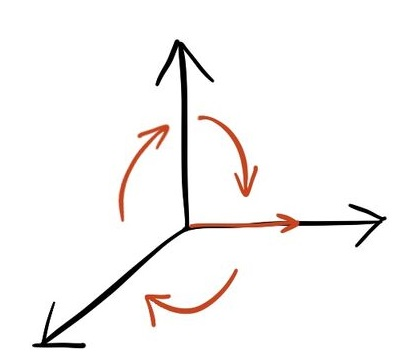
\includegraphics[width=0.4\textwidth]{C:/Users/Nacho/Documents/Latex/Facultad/GeometriaProyectiva/GeoProyectiva/rotacionfijae1.jpg}
	\caption{Una rotación en $\RR^3$ que deja fijo al eje $e_1$}
	\label{fig:rotacionfijae1}
\end{figure}

Para $n=2$, sabemos que $A^{-1}$ queda unívocamente determinada como la matriz cuyas columnas son $\tau(\sigma,s_0)$ y $\eta(\sigma,s_0)$ y si $W(0,e_1)=ae_1 + be_2$, obtenemos que $$V(\sigma,s_0)=A^{-1}W(0,e_1) = a\tau(\sigma,s_0)+b\eta(\sigma,s_0)$$ que es fácil comprobar que es un invariante (pues el par $\{\tau(\sigma,s_0),\eta(\sigma,s_0)\}$ forma siempre una base ortonormal con determinante $1$). Y estamos.
\end{proof}
\end{prop}

Por último, vamos a caracterizar los invariantes diferenciales escalares de orden $2$. Para ello, antes consideremos la siguiente definición:

\begin{defn}
Sea $(\sigma,s_0)\in\mathscr{C}(n)$. Se define la \textbf{curvatura} de $\sigma$ en $s_0$ como: $$\kappa(\sigma,s_0)=\dfrac{\sqrt{\norm{\sigma'(s_0)}^2\norm{\sigma''(s_0)}^2 - \langle\sigma'(s_0),\sigma''(s_0)\rangle^2}}{\norm{\sigma'(s_0)}^3}$$
\end{defn}

Notemos que la curvatura $\kappa(\sigma,s_0)$ es un invariante diferencial escalar de orden $2$. En efecto, si $f:\RR^n\to\RR^n$, $f\in\Iso^+(n)$, entonces tenemos que $(f\circ\sigma)'(s_0)=A_f\sigma'(s_0)$ y $(f\circ\sigma)''(s_0)=A_f\sigma''(s_0)$, y reemplazando en la fórmula de la curvatura (y notando que $A_f\in\mathrm{SO}(n)$ y así preserva ángulos y distancias), es claro que $\kappa(f\circ\sigma,s_0)=\kappa(\sigma,s_0)$. Por otra parte, si $u:(c,d)\to\mathrm{Dom}\sigma$ es una reparametrización directa, por la regla de la cadena es fácil ver que se tiene $(\sigma\circ u)'(u^{-1}(s_0)) = \sigma'(s_0)u'(u^{-1}(s_0))$ y también tenemos $(\sigma\circ u)''(u^{-1}(s_0)) = \sigma''(s_0) u'(u^{-1}(s_0))^2 + \sigma'(s_0)u''(u^{-1}(s_0))$. Es fácil comprobar, usando esto, que $\kappa(\sigma\circ u,u^{-1}(s_0)) = \kappa(\sigma,s_0)$. Notemos también que si $\varphi:\RR_{>0}\to\RR$ es una función cualquiera, entonces $\varphi(\kappa(\sigma,s_0))$ también es un invariante diferencial escalar de orden $2$. Veamos que vale la recíproca:

\begin{prop}
Sea $V$ un invariante diferencial escalar de orden $2$. Entonces, existe una función $\varphi:\RR_{>0}\to\RR$ tal que $V(\sigma,s_0)=\varphi(\kappa(\sigma,s_0))$.
\begin{proof}
Consideremos $A\in\mathrm{SO}(n)$ tal que $A\sigma'(s_0)=\norm{\sigma'(s_0)}e_1$, la traslación ${f:\RR^n\to\RR^n}$ dada por $f(x)=A(x-\sigma(s_0))$ y la reparametrización $u(s)=s_0+\dfrac{s-s_0}{\norm{\sigma'(s_0)}}$. Es claro que $u^{-1}(s_0)=s_0$. Considero entonces $\gamma = f\circ\sigma\circ u$. Como $V$ es un invariante, tenemos que $V(\gamma,s_0)=V(f\circ\sigma\circ u,s_0)=V(\sigma\circ u,s_0)=V(\sigma,s_0)$. Pero tenemos que $\gamma(s_0)=0$, $\gamma'(s_0)=e_1$ y así $V(\gamma,s_0)=W(0,e_1,\gamma''(s_0))$, donde $W:(\RR^n)^3\to\RR$ es la función tal que $V(\sigma,s_0)=W(\sigma(s_0),\sigma'(s_0),\sigma''(s_0))$. 

Sea $M\in\mathrm{SO}(n)$ una rotación con eje $e_1$ (es decir, $Me_1=e_1$). Entonces, si $g:\RR^n\to\RR^n$, $g(x)=Mx$, se cumple que $W(0,e_1,M\gamma''(s_0))=V(g\circ\gamma,s_0)=V(\gamma,s_0)=W(0,e_1,\gamma''(s_0))$. Por otra parte, supongamos que $u:(a,b)\to\mathrm{Dom}\sigma$ es una reparametrización directa tal que $s_0\in (a,b)$, $u(s_0)=s_0$ y $u'(s_0)=1$. Entonces, por la regla de la cadena, tenemos que $W(0,e_1,u''(s_0)\gamma'(s_0)+\gamma''(s_0)) = V(\gamma\circ u,s_0)=V(\gamma,s_0)=W(0,e_1,\gamma''(s_0))$. En resumen, si definimos $\Phi(v)=W(0,e_1,v)$, tendremos que $\Phi(A\gamma''(s_0))=\Phi(\gamma''(s_0))$ para toda ${M\in\mathrm{SO}(n)}$ tal que $Me_1=e_1$, y tendremos que $\Phi(u''(s_0)e_1+\gamma''(s_0))=\Phi(\gamma''(s_0))$ para toda reparametrización $u$ tal que $u(s_0)=s_0$ y $u'(s_0)=1$.

Si consideramos la curva $\gamma(s)=(s-s_0)e_1 + \dfrac{(s-s_0)^2}{2}v$, con $v\in\RR^n$, se tiene que $\gamma'(s_0)=e_1\neq 0$ y así define una curva regular en un entorno de $s_0$. Como los invariantes están definidos a menos del germen, podemos mirar $V(\gamma,s_0)$. Esta curva $\gamma$ cumple que $\gamma(s_0)=0$, $\gamma'(s_0)=e_1$ y $\gamma''(s_0)=v$. Por lo tanto, $\Phi(v)=\Phi(Mv)$ para toda $M\in\mathrm{SO}(n)$ tal que $Me_1=e_1$. Ahora, consideremos la reparametrización $u_\lambda(s)=s_0 + \lambda\dfrac{(s-s_0)^2}{2}$, definida en un entorno de $s_0$. Luego, tenemos que $\Phi(\lambda e_1 + v)=\Phi(v)$. Es decir, $\Phi$ es constante sobre cilindros con eje $e_1$. Por lo tanto, para definir $\Phi(v)$ sólo nos importa la norma de su proyección ortogonal sobre $\langle e_1\rangle^{\perp}$. Esto implica que existe $\varphi:\RR_{>0}\to\RR$ tal que $\Phi(v)=\varphi(\norm{v-\pint{v,e_1}e_1})$ para todo $v\in\RR^n$.

Ahora bien, juntando todo lo que hicimos, tenemos la siguiente fórmula: $$V(\sigma,s_0)=W(0,e_1,\gamma''(s_0))=\Phi(\gamma''(s_0))=\varphi(\norm{\gamma''(s_0)+\pint{\gamma''(s_0),e_1}e_1})$$ donde $\gamma(s)=f\circ\sigma\circ u(s)$ como en el primer párrafo. Es fácil comprobar, por la regla de la cadena, que $\gamma''(s_0)=A\dfrac{\sigma''(s_0)}{\norm{\sigma'(s_0)}^2}$. Además, notemos que como $A\sigma'(s_0) = \norm{\sigma'(s_0)}e_1$, se tiene que $A\dfrac{\sigma'(s_0)}{\norm{\sigma'(s_0)}} = e_1$. Estamos en condiciones de calcular la norma de la proyección ortogonal de $\gamma''(s_0)$. Simplemente es escribir todo y usar que $A\in\mathrm{SO}(n)$ preserva ángulos y distancias. En efecto: \begin{align*}\norm{\gamma''(s_0)+\pint{\gamma''(s_0),e_1}e_1} &= \norm{A\dfrac{\sigma''(s_0)}{\norm{\sigma'(s_0)}^2} - \pint{A\dfrac{\sigma''(s_0)}{\norm{\sigma'(s_0)}^2},A\dfrac{\sigma'(s_0)}{\norm{\sigma'(s_0)}}}A\dfrac{\sigma'(s_0)}{\norm{\sigma'(s_0)}}} \\ &= \norm{A\left(\dfrac{\sigma''(s_0)}{\norm{\sigma'(s_0)}^2} - \pint{A\dfrac{\sigma''(s_0)}{\norm{\sigma'(s_0)}^2},A\dfrac{\sigma'(s_0)}{\norm{\sigma'(s_0)}}}\dfrac{\sigma'(s_0)}{\norm{\sigma'(s_0)}}\right)}\\&= \norm{\dfrac{\sigma''(s_0)}{\norm{\sigma'(s_0)}^2} - \pint{\dfrac{\sigma''(s_0)}{\norm{\sigma'(s_0)}^2},\dfrac{\sigma'(s_0)}{\norm{\sigma'(s_0)}}}\dfrac{\sigma'(s_0)}{\norm{\sigma'(s_0)}}} \\ &= \dfrac{\norm{\sigma''(s_0)\norm{\sigma'(s_0)}^2 - \pint{\sigma'(s_0),\sigma''(s_0)}\sigma'(s_0)}}{\norm{\sigma'(s_0)}^4}\\&=\dfrac{\sqrt{\norm{\sigma''(s_0)^2}\norm{\sigma'(s_0)}^4 -\norm{\sigma'(s_0)}^2\pint{\sigma'(s_0),\sigma''(s_0)}^2}}{\norm{\sigma'(s_0)}^4} \\ &= \dfrac{\sqrt{\norm{\sigma'(s_0)}^2\norm{\sigma''(s_0)}^2 - \pint{\sigma'(s_0),\sigma''(s_0)}^2}}{\norm{\sigma'(s_0)}^3}\end{align*}Es decir, hemos probado que $\norm{\gamma''(s_0)+\pint{\gamma''(s_0),e_1}e_1} = \kappa(\sigma,s_0)$. Como ya habíamos visto que $V(\sigma,s_0)=\varphi(\norm{\gamma''(s_0)+\pint{\gamma''(s_0),e_1}e_1})$, esto nos dice que $V(\sigma,s_0)=\varphi(\kappa(\sigma,s_0))$. Esto concluye la demostración.
\end{proof}
\end{prop}

Consideremos por un momento invariantes escalares de curvas planas. Es decir, invariantes $V:\mathscr{C}(2)\to\RR$. Sea $(\sigma,s_0)\in\mathscr{C}(2)$, con $\sigma:(a,b)\to\RR^n$. Podemos considerar $V_\sigma:(a,b)\to\RR$ definida por $V_\sigma(s)=V(\sigma,s)$. Decimos que $V$ es un invariante \textbf{diferenciable} si existe la derivada $\left.\dfrac{\mathrm{d}}{\mathrm{ds}}\right\rvert_{s=s_0} V_\sigma(s)$. Claramente, la derivada está bien definida en el germen (pues si $(\sigma,s_0)\sim(\tau,t_0)$ entonces $\sigma$ y $\tau$ coincidirán en un entorno de $s_0=t_0$ y así $V_\sigma$ y $V_\tau$ también). Consideremos entonces la asignación $U:\mathscr{C}(2)\to\RR$ dada por $U(\sigma,s_0)=\left.\dfrac{\mathrm{d}}{\mathrm{ds}}\right\rvert_{s=s_0} V_\sigma(s)$. Usando que $V$ es invariante, es fácil ver que $U(f\circ\sigma,s_0)=U(\sigma,s_0)$ para $f\in\Iso^+(n)$. Ahora, si $u:(c,d)\to\mathrm{Dom}\sigma$ es una reparametrización, tenemos que: \begin{align*}U(\sigma\circ u,u^{-1}(s_0)) = \left.\dfrac{\mathrm{d}}{\mathrm{dt}}\right\rvert_{t=u^{-1}(s_0)} V(\sigma\circ u,t)&=\left.\dfrac{\mathrm{d}}{\mathrm{dt}}\right\rvert_{t=u^{-1}(s_0)} V(\sigma,u(t))\\ &= u'(u^{-1}(s_0)) \left.\dfrac{\mathrm{d}}{\mathrm{ds}}\right\rvert_{s=s_0} V(\sigma,s)\\ &= U(\sigma,s_0)u'(u^{-1}(s_0))\end{align*} Es decir, $U$ \textbf{no} es un invariante, pero casi. Simplemente consideremos: $$DV(\sigma,s_0) = \dfrac{1}{\norm{\sigma'(s_0)}^2}\left.\dfrac{\mathrm{d}}{\mathrm{ds}}\right\rvert_{s=s_0} V_\sigma(s)$$ Esto es un invariante pues $\norm{\sigma'(s_0)}$ permanece invariante bajo movimientos euclídeos y con reparametrizaciones también aparece un factor $u'(u^{-1}(s_0))$ que se cancela con el de $U$. Es decir, construimos un invariante $DV$ a partir de $V$. Si $V$ es un invariante diferencial de orden a lo sumo $d$, entonces $DV$ debería ser de orden a lo sumo $d+1$ (pues escribimos $V(\sigma,s_0)=W(\sigma(s_0),\ldots,\sigma^{(d)}(s_0))$ y derivamos usando la regla de la cadena, si asumimos alguna condición de regularidad en $W$).

Ahora bien, en $\mathscr{C}(2)$ nosotros conocemos dos invariantes: la tangente $\tau$ y la normal $\eta$. Notemos que como $\norm{\tau(\sigma,s)}^2 = 1$ para todo $s$, derivando el producto interno se sigue que $2\pint{\tau(\sigma,s_0),\left.\dfrac{\mathrm{d}}{\mathrm{ds}}\right\rvert_{s=s_0}\tau(\sigma,s)} = 0$ para todo $s_0$. Esto implica que para cualquier $s_0$ tenemos que $\eta(\sigma,s_0)$ es paralelo a $D\tau(\sigma,s_0)=\left.\dfrac{\mathrm{d}}{\mathrm{ds}}\right\rvert_{s=s_0} \tau(\sigma,s)$. Por lo tanto, debemos tener que $D\tau(\sigma,s_0) = \pint{D\tau(\sigma,s_0),\eta(\sigma,s_0)}\eta(\sigma,s_0)$. Pero notemos que $\pint{D\tau(\sigma,s_0),\eta(\sigma,s_0)}$ es un invariante diferencial escalar de orden menor o igual que $2$, y por ende debe ser de la forma $\varphi(\kappa(\sigma,s_0))$ para alguna $\varphi:\RR_{>0}\to\RR$. Es decir, para todo $(\sigma,s_0)\in\mathscr{C}(2)$ se tiene que $D\tau(\sigma,s_0)=\varphi(\kappa(\sigma,s_0))\eta(\sigma,s_0)$. Entonces, si consideramos las circunferencias $\sigma_r:\RR\to\RR^2$, $\sigma_r(t)=(r\cos t,r\sen t)$ para $r>0$, es fácil ver que $\kappa(\sigma_r,s)=\dfrac{1}{r}$ para todo $s\in\RR$. Además, como $\tau(\sigma_r,s)=(-\sen s,\cos s)$, $\eta(\sigma_r,s)=-(\cos s,\sen s)$, se sigue que $D\tau(\sigma,s)=\dfrac{1}{\norm{\sigma''(s_0)}}(-\cos s,\sen s) = \dfrac{1}{r}(-\cos s,\sen s) = \dfrac{1}{r}\eta(\sigma,s)$. Por lo tanto, tenemos que $\varphi\left(\dfrac{1}{r}\right)=\dfrac{1}{r}$ para todo $r>0$, que implica $\varphi(x)=x$. 

Hemos probado que $D\tau(\sigma,s_0)=\kappa(\sigma,s_0)\eta(\sigma,s_0)$. De manera análoga, podemos probar la relación $D\eta(\sigma,s_0)=-k(\sigma,s_0)\tau(\sigma,s_0)$. Ahora bien, la primera relación se puede escribir como $\tau' = \norm{\sigma'}\kappa\eta$, y como $\tau = \dfrac{\sigma'}{\norm{\sigma'}}$, derivando podemos expresar a $\sigma''$ en términos de $\sigma',\tau,\kappa$ y $\eta$. Procediendo así sucesivamente, podemos expresar a todas las derivadas de orden superior en términos de estos elementos, y así los únicos invariantes diferenciales relevantes en el plano son $\tau,\eta$ y $\kappa$.



